\documentclass[12pt,a4paper]{report}

\usepackage{anysize}
% \marginsize{3.81cm}{2.54cm}{2.54cm}{2.54cm} % use this margin for printing
\marginsize{2.54cm}{2.54cm}{2.54cm}{2.54cm} % use this margin for viewing

\usepackage{graphicx}
\graphicspath{{figures/}}

\usepackage{fontspec}
\setmainfont{Times New Roman}

\usepackage{url}

\usepackage[nottoc]{tocbibind} % show bibiliography in table of contents without numbering

\usepackage[titles]{tocloft}
% add dots to table of content
\renewcommand{\cftchapleader}{\cftdotfill{\cftdotsep}} % for chapters
\renewcommand{\cftsecleader}{\cftdotfill{\cftdotsep}} % for sections

\renewcommand{\appendixname}{APPENDIX} % change the name before using the appendix package
\usepackage{appendix}


\usepackage{titlesec}
% centering chapter title and remove page number of the first page of every chapter
 % use \chaptertitlename to add chapter or appendix prefix automatically
\makeatletter
\titleformat{\chapter}[hang]
  {\large\bfseries\filcenter}
  {\MakeUppercase{\chaptertitlename}~\thechapter:~}
  {0em}
  {\thispagestyle{empty}}
\makeatother


% formatting section, subsection and subsubsection title
\titleformat{\section}
{\large\bfseries}{\thesection~}{0em}{\MakeUppercase}

\titleformat{\subsection}
{\normalsize\bfseries}{\thesubsection~}{0em}{\MakeUppercase}

\titleformat{\subsubsection}
{\normalsize\bfseries}{}{0em}{\MakeLowercase}

% add chapter prefix to table of contents
\renewcommand{\cftchappresnum}{\MakeUppercase{\chaptertitlename}~}
\renewcommand{\cftchapaftersnum}{:}
\newlength{\toclen}
\settowidth{\toclen}{\cftchappresnum\cftchapaftersnum}
\addtolength{\cftchapnumwidth}{\toclen}

% \makeatletter
% \g@addto@macro\appendix{%
%   \addtocontents{toc}{%
%     \protect\renewcommand{\protect\cftchappresnum}{APPENDIX~}%
%     \renewcommand{\cftchapaftersnum}{:}
%     \newlength{\toclen}
%     \settowidth{\toclen}{\cftchappresnum\cftchapaftersnum}
%     \addtolength{\cftchapnumwidth}{\toclen}
%   }%
% }
% \makeatother

% set font style in table of contents
\renewcommand{\cftchapfont}{\normalsize\rmfamily}
\renewcommand{\cftsecfont}{\normalsize\rmfamily}
\renewcommand{\cftsubsecfont}{\normalsize\rmfamily}
\renewcommand{\cftfigfont}{\normalsize\rmfamily}
\renewcommand{\cfttabfont}{\normalsize\rmfamily}
\renewcommand{\cftchappagefont}{\normalsize\rmfamily}

% add Figure prefix
\newlength{\loflen}
\renewcommand{\cftfigpresnum}{\figurename~}
\renewcommand{\cftfigaftersnum}{:}
\renewcommand{\cftfigindent}{0em}
\settowidth{\loflen}{\cftfigpresnum\cftfigaftersnum}
\addtolength{\cftfignumwidth}{\loflen}

% add Table prefix
\newlength{\lotlen}
\renewcommand{\cfttabpresnum}{\tablename~}
\renewcommand{\cfttabaftersnum}{:}
\renewcommand{\cfttabindent}{0em}
\settowidth{\lotlen}{\cfttabpresnum\cfttabaftersnum}
\addtolength{\cfttabnumwidth}{\lotlen}

\usepackage[toc,acronyms,nonumberlist,nopostdot]{glossaries}
\makenoidxglossaries
% \makeglossaries
\newglossaryentry{Word 1}
{
  name=Word 1,
  description={The first word in glossary}
}

\newglossaryentry{Word 2}
{
  name=Word 2,
  description={The second word in glossary}
}

\newglossaryentry{Word 3}
{
  name=Word 3,
  description={The third word in glossary}
}

\newacronym{abrv1}{ABRV1}{Abbreviation1}

\newacronym{abrv2}{ABRV2}{Abbreviation2}

\newacronym{abrv3}{ABRV3}{Abbreviation3, balabalabala}
% \loadglsentries{contents/glossary}

\usepackage{multirow}
\usepackage{float} % allow the use of H for positioning

\usepackage{setspace}
\onehalfspacing

\setlength{\parindent}{0pt} % no indent

\setcounter{tocdepth}{2} % no subsubsection in table of contents

\usepackage[hang,flushmargin]{footmisc} % no footnote indentation

\renewcommand{\contentsname}{\hfill\large\bfseries TABLE OF CONTENTS\hfill}
\renewcommand{\cftaftertoctitle}{\hfill}

\renewcommand{\listfigurename}{\normalsize\rmfamily LIST OF FIGURES}

\renewcommand{\listtablename}{\normalsize\rmfamily LIST OF TABLES}

\renewcommand{\bibname}{BIBILIOGRAPHY}

% remove numbering of section and subsection in table of contents
% \makeatletter
% \let\latexl@section\l@section
% \def\l@section#1#2{\begingroup\let\numberline\@gobble\latexl@section{#1}{#2}\endgroup}
% \makeatother

% \makeatletter
% \let\latexl@subsection\l@subsection
% \def\l@subsection#1#2{\begingroup\let\numberline\@gobble\latexl@subsection{#1}{#2}\endgroup}
% \makeatother

\begin{document}
\thispagestyle{empty}
\begin{titlepage}
    \begin{center}
        \bigskip
        \bigskip
        \Large \textbf{Thesis Title}\\
        \bigskip by\\
        \begin{spacing}{2}
            \textbf{Author Name}\\
        \end{spacing}
        \vfill
        % \begin{spacing}{1.5}
            Degree Title\\
            % \vspace{0.8cm}
            \vfill
            \date{Day Month Year}
        % \end{spacing}
        
\includegraphics[width=0.3\textwidth]{UM_Logo}\\
        \begin{spacing}{1}
            \Large
            \textbf{Faculty of Science and Technology}\\
            \textbf{University of Macau}
        \end{spacing}
    \end{center}
\end{titlepage}
\newpage
\thispagestyle{empty}
\begin{titlepage}
  \begin{center}
    Thesis Title\\
    % \vspace{1cm}by\vspace{1cm}\\
    % Author Name\\
    % \vspace{1cm}
    \begin{spacing}{2}
      by\\
      Author Name\\\
    \end{spacing}
    % A thesis submitted in partial fulfillment of\\
    % the requirements for the degree of\\
    % \vspace{1cm}
    \begin{spacing}{1}
      A thesis submitted in partial fulfillment of\\
      the requirements for the degree of\\
    \end{spacing}
    \bigskip
    \bigskip
    Degree Type\\
    % \vspace{1cm}
    % Faculty of Science and Technology\\
    % University of Macau\\
    % \vspace{1cm}
    \bigskip
    \bigskip
    \begin{spacing}{1}
      Faculty of Science and Technology\\
      University of Macau\\
    \end{spacing}
    \bigskip
    \bigskip
    Year
  \end{center}
  \vfill
  Approved by \hrulefill\\ % \underline{\hspace{0.9\textwidth}}
  \centerline{Supervisor}
  % \begin{spacing}{2}
  \hphantom{invisible line}\\
  \bigskip
  \hphantom{Approved by} \hrulefill\\
  \bigskip
  \hphantom{Approved by} \hrulefill\\
  \bigskip
  \hphantom{Approved by} \hrulefill\\
  % \end{spacing}
  % \begin{flushright}
  %   \begin{minipage}[position]{0.8\textwidth}
  %     \hrulefill\\
  %     \bigskip
  %     \bigskip
  %     \hrulefill\\
  %     \bigskip
  %     \bigskip
  %     \hrulefill\\
  %   \end{minipage}
    % \underline{\hspace{\textwidth}}
    % \underline{\hspace{\textwidth}}
    % \underline{\hspace{\textwidth}}
  % \end{flushright}
  Date \hrulefill % \underline{\hspace{\textwidth}}
\end{titlepage}

\newpage
\thispagestyle{empty}
\noindent In presenting this thesis in partial fulfillment of the requirements for a Master's degree at the University of Macau, I agree that the Library and the Faculty of Science and Technology shall make its copies freely available for inspection. However, reproduction of this thesis for any purposes or by any means shall not be allowed without my written permission. Authorization is sought by contacting the author at\\
% \setlist{nolistsep} % by enumitem package
% \begin{description}[font=\normalfont]
%   \item[Address:] \hphantom{invisible line}
%   \item[Telephone:] \hphantom{invisible line}
%   \item[Fax:] \hphantom{invisible line}
%   \item[E-mail:] \hphantom{invisible line}
% \end{description}
\hphantom{invisible line}\\
\hphantom{indent}Address:\\
\hphantom{indent}Telephone:\\
\hphantom{indent}Fax:\\
\hphantom{indent}E-mail:\\
\hphantom{invisible line}
\hphantom{invisible line}
\begin{flushright}
  \begin{minipage}[position]{0.5\textwidth}
    Signature \hrulefill\\ % \underline{\hspace{0.8\textwidth}}\\
    \hphantom{invisible line}\\
    Date \hrulefill % \underline{\hspace{0.8\textwidth}}
  \end{minipage}
  % \makebox[0.4\textwidth][]{%
  %   Signature \underline{\hspace{\textwidth}}\\
  %   Date \underline{\hspace{\textwidth}}
  % }
\end{flushright}
\newpage
\thispagestyle{empty}
\begin{center}
  \begin{spacing}{2}
    University of Macau\\
    Abstract\\
  \end{spacing}
  Title\\
  \begin{spacing}{2}
    by Name\\
  \end{spacing}
  Thesis Supervisor:\\
  Title and supervisor name\\
  Program name\\
\end{center}
\hphantom{invisible line}
The Faculty requires an Abstract for a master's or doctoral thesis.  It must be in both submitted copies and must follow the format given in the sample. The title of the thesis must appear exactly as it does on the Title Page. The name of your Supervisor must appear in full with his or her appropriate academic title (no professional titles may be used) and the name of the program authorized to offer the degree.

The text of the Abstract must be one-and-one-half or double-spaced and must conform to margin requirements.

All abstracts must not exceed 350 words or 35 lines (this requirement is inline with the requirement of Dissertation Abstracts International so that your abstract could be published in full there if necessary).

It is requested by the publisher that the Abstract not include formulas, diagrams, or symbols. Should a formula, diagram, or symbol be essential to the text in the Abstract, it may not be handwritten. If Greek letters of the alphabet are to be used, they must be clearly inscribed.

\newpage
\pagenumbering{roman}
% \thispagestyle{empty}
% \begin{spacing}{1}
\tableofcontents
% \end{spacing}
\newpage
\thispagestyle{plain}
\listoffigures
\addtocontents{lof}{{\textit{Number}}~\hfill{\textit{Page}}\par}
\newpage
\thispagestyle{plain}
\listoftables
\addtocontents{lot}{{\textit{Number}}~\hfill{\textit{Page}}\par}
\newpage
\thispagestyle{plain}
% \printglossary[title=Glossary,toctitle=Glossary]
% \printglossary[type=\acronymtype,title=LIST OF ABBREVIATIONS,toctitle=LIST OF ABBREVIATIONS]
% \glsaddall
\printnoidxglossaries
% \glsaddall
% \printglossaries
% \printnoidxglossaries[type=\acronymtype]
\newpage
\addcontentsline{toc}{chapter}{PREFACE}
\newpage
\chapter*{PREFACE}
\thispagestyle{plain}
\newpage
\newpage
\chapter*{ACKNOWLEDMGENTS}
\thispagestyle{plain}
The author wishes to \dots

Acknowledgments recognize the persons to whom you are indebted for guidance and assistance and those to whom you are grateful for any special or non-routine aid. Faculty members serve on Examination Committees as part of their regular work and do not require formal acknowledgment, although in most cases the help given far exceeds any requirement and should, as a matter of courtesy, be recognized.

Acknowledgments should be expressed simply and tactfully. They should be one-and-one-half or double-spaced and conform with margin requirements.
\newpage
\newpage
\chapter*{DEDICATION}
\thispagestyle{plain}
The author wishes to dedicate this thesis to \dots
\newpage
\pagenumbering{arabic}
\chapter{REMAINING WORK}
\begin{itemize}
  \item move preamble to a class file
  \item show page numbers for List of Figures, List of Tables, Glossary and Acronyms
  \item convert all entries in Table of Content to uppercase
  \item correct the order of words in Glossary
  \item correct the prefix of appendix entries in Table of Contents
  \item convert the title of Glossary and Acronyms to uppercase
\end{itemize}
\chapter{DUMMY CHAPTER}
\begin{figure}[H]
  \centering
  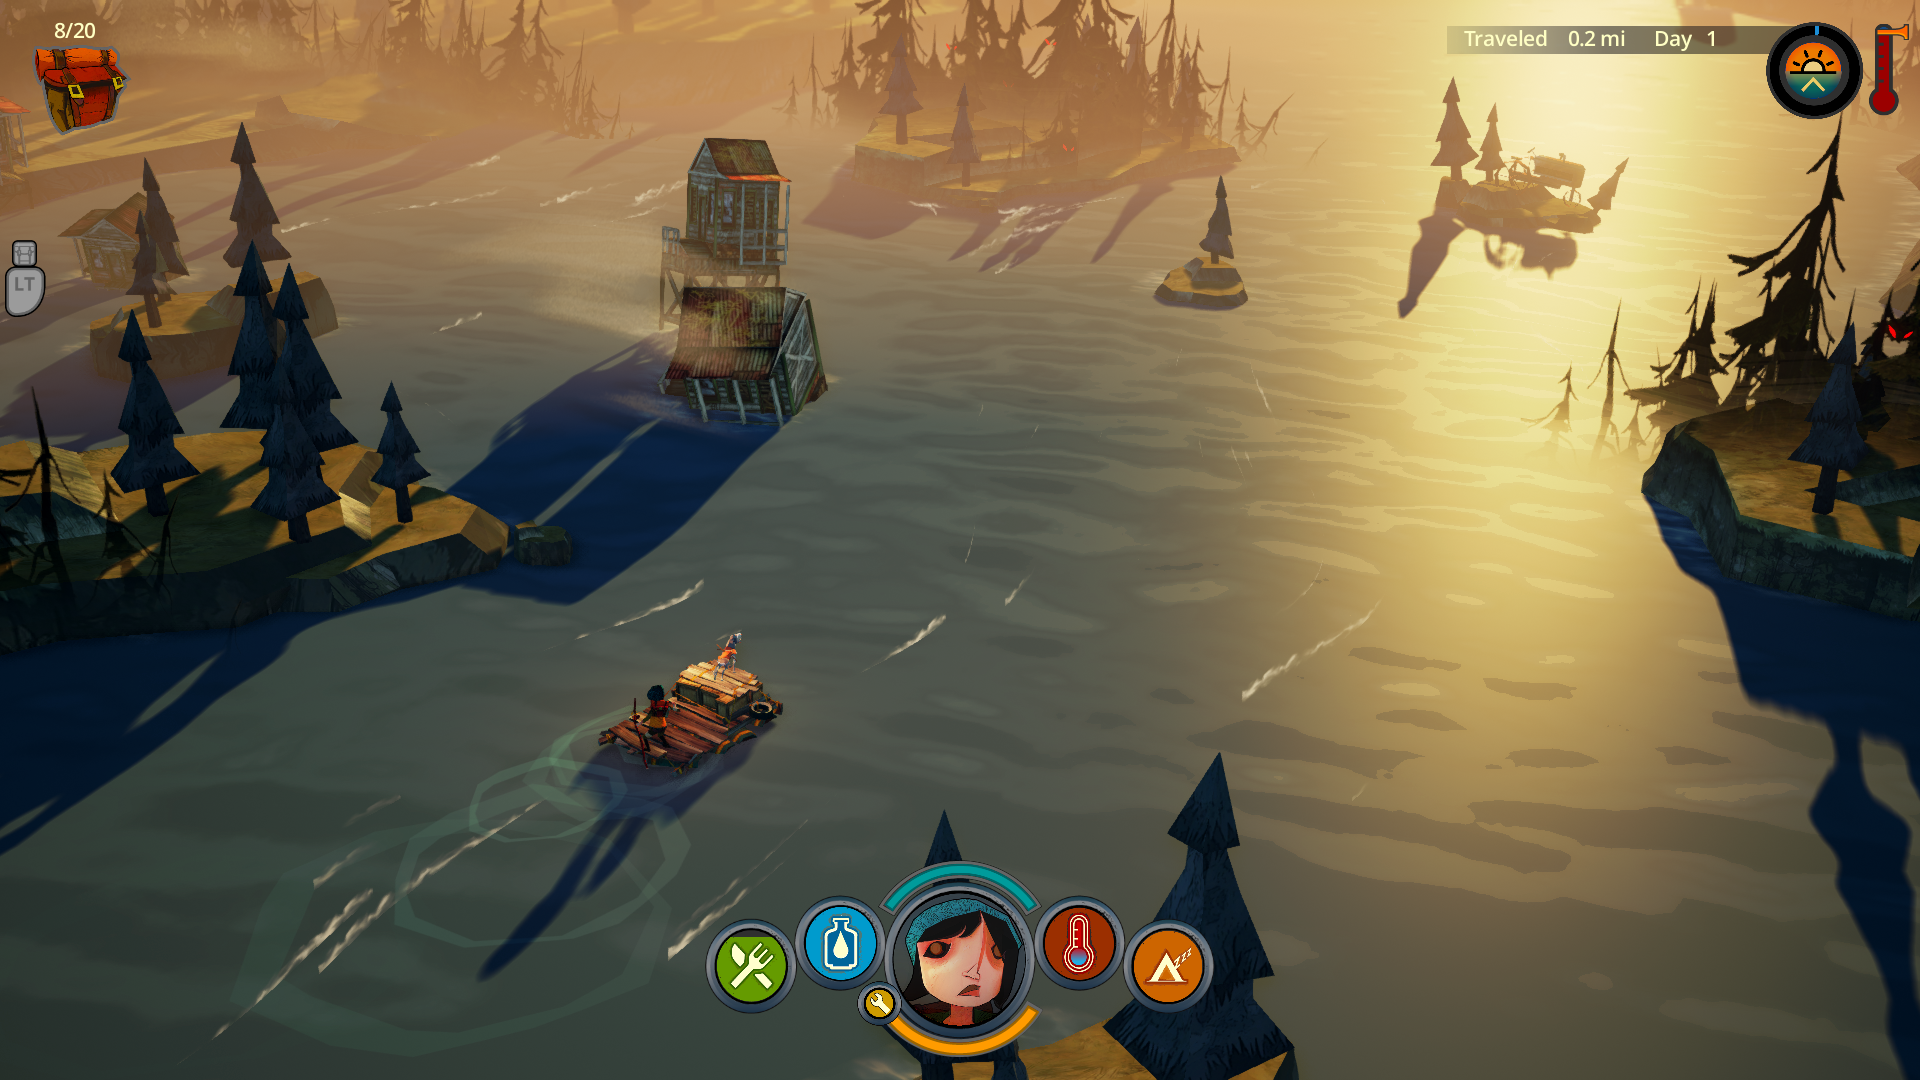
\includegraphics[width=0.4\linewidth]{flame_flood.png}
  \caption{A screenshot}\label{fig:1}
\end{figure}
There is a figure above: Figure~\ref{fig:1}
\chapter{ANOTHER CHAPTER}
chapter text here
\section{SECTION SAMPLE}
Long acronym: \acrlong{abrv1}\\
Short acronym: \acrshort{abrv2}\\
Full acronym: \acrfull{abrv3}
\subsection{SUBSECTION SAMPLE}
some words:
\begin{itemize}
  \item lower case: \gls{Word 1}
  \item sentence case:\Gls{Word 2}
  \item lower case plural form: \glspl{Word 1}
  \item sentence case plural form:\Glspl{Word 1}
\end{itemize}

Cite something~\cite{online1}

Cite misc~\cite{misc1}

Cite article~\cite{article1}

Cite incollection~\cite{incollection1}

text with footnote~\footnote{Footnote with url: \url{https://link/to/some/site}}.

\subsubsection{a subsubsection}
\begin{table}[H]
  \centering
  \caption{Sample Table}\label{tab:1}
  \begin{tabular}{|c|c|c|c|}
    \hline
    \multicolumn{2}{|c|}{}&\multicolumn{2}{c|}{Some text}\\
    \cline{3-4}
    \multicolumn{2}{|c|}{}&Yes&No\\
    \hline
    \multirow{2}{*}{text}&text&text&text\\
    \cline{2-4}
    &text&text&text\\
    \hline
  \end{tabular}
\end{table}

There is a table above: Table~\ref{tab:1}

\bibliography{contents/reference}
\bibliographystyle{IEEEtran}
\begin{appendices}
  \chapter{APPENDIX SAMPLE}
Appendices may consist of material that is related to, but not appropriate for, inclusion in the text. They appear after the Bibliography or List of References and must be titled. They are listed, along with their titles, in the Table of Contents, not on a separate list of appendices. Pagination is continuous with the text, and the first page of each appendix is treated like the first page of a chapter in the text (i.e., counted, but not numbered).

  \chapter{MORE APPENDIX SAMPLE}
Appendix material also need to meet the requirements for margins and readability. Material may be reduced as long as it remains legible. However, appendix titles and page numbers must remain full-size; it is recommended that they be added to the page after reduction.
  \chapter{ANOTHER APPENDIX SAMPLE}
Any illustrations appearing in the appendices which are not from previously published material must be captioned and placed in the appropriate list.

\end{appendices}
% \appendix
%   \chapter{APPENDIX SAMPLE}
Appendices may consist of material that is related to, but not appropriate for, inclusion in the text. They appear after the Bibliography or List of References and must be titled. They are listed, along with their titles, in the Table of Contents, not on a separate list of appendices. Pagination is continuous with the text, and the first page of each appendix is treated like the first page of a chapter in the text (i.e., counted, but not numbered).

%   \chapter{MORE APPENDIX SAMPLE}
Appendix material also need to meet the requirements for margins and readability. Material may be reduced as long as it remains legible. However, appendix titles and page numbers must remain full-size; it is recommended that they be added to the page after reduction.
%   \chapter{ANOTHER APPENDIX SAMPLE}
Any illustrations appearing in the appendices which are not from previously published material must be captioned and placed in the appropriate list.

\end{document}